%%%%%%%%%%%%%%%%%%%%%%%%%%%%%%%%%%%%%%%%%
% University/School Laboratory Report
% LaTeX Template
% Version 4.0 (March 21, 2022)
%
% This template originates from:
% https://www.LaTeXTemplates.com
%
% Authors:
% Vel (vel@latextemplates.com)
% Linux and Unix Users Group at Virginia Tech Wiki
%
% License:
% CC BY-NC-SA 4.0 (https://creativecommons.org/licenses/by-nc-sa/4.0/)
%
%%%%%%%%%%%%%%%%%%%%%%%%%%%%%%%%%%%%%%%%%

%----------------------------------------------------------------------------------------
%	PACKAGES AND DOCUMENT CONFIGURATIONS
%----------------------------------------------------------------------------------------

\documentclass[
	a4paper, % Paper size, specify a4paper (A4) or letterpaper (US letter)
	11pt, % Default font size, specify 10pt, 11pt or 12pt
]{CSUniSchoolLabReport}

\addbibresource{sample.bib} % Bibliography file (located in the same folder as the template)

\usepackage{subcaption}
\usepackage{siunitx}

%----------------------------------------------------------------------------------------
%	REPORT INFORMATION
%----------------------------------------------------------------------------------------

\title{항공기 날개 공력탄성학 및 플러터 진동 해석\\
120520-1} % Report title

\author{김세경\\C417025} % Author name(s), add additional authors like: '\& James \textsc{Smith}'

\date{\today} % Date of the report

%----------------------------------------------------------------------------------------

\begin{document}

\maketitle % Insert the title, author and date using the information specified above

% \begin{center}
% 	\begin{tabular}{l r}
% 		Date Performed: & February 13, 2022 \\ % Date the experiment was performed
% 		Partners: & Cecilia \textsc{Smith} \\ % Partner names
% 		& Tajel \textsc{Khumalo} \\
% 		Instructor: & Professor \textsc{Rivera} % Instructor/supervisor
% 	\end{tabular}
% \end{center}

% If you need to include an abstract, uncomment the lines below
%\begin{abstract}
%	Abstract text
%\end{abstract}
\section{개요}
항공기의 날개는 이륙과 착륙과정에서 가장 큰 스트레스를 겪는다.하지만 이를 제외하고도, 순항과정에서도 여러 요인에 의하여
지속적으로 스트레스를 받으며 항공기가 최대효율을 내며 비행하는것을 제한한다.
이 중 연비에 가장 큰 영향을 미치는 순항속도에 있어서,그것을 제한하는 첫번째 요소인 Flutter 현상을 해결하는 것이 연비 향상에 큰 도움이 된다.
이를 공력탄성학적인 시선에서 접근하여, 항공기 날개의 공력탄성학적 특성을 해석하고, Flutter 현상을 예측하여, 
항공기 날개를 위한 최소한의 디자인을 제시해보고자 한다.
%----------------------------------------------------------------------------------------
%	Model and state space definitions
%----------------------------------------------------------------------------------------

\section{시스템 모델 및 상태공간,전달함수 정의}
\subsection{모델 간소화 및 자유도 축소}
해당 탐구에서는 해석을 용이하게 하기위한,그리고  자원의 한계로 다음과 같은 가정하에서 프로젝트를 진행하였다.
\begin{enumerate}
	\item 날개는 대칭적이고 균일한 구조이다
	\item 날개의 길이는 무한하다. Wing vortex 등 유한한 길이의 날개로 인한 효과는 무시하며, 2차원 익형 해석으로 진행한다.
	\item 날개의 길이 방향으로 인한 탄성학적 효과는 익형에 달려있는 두개의 스프링,두개의 댐퍼로 근사할 수 있다 
	\item 해당 가상 실험은 풍동 내부에서 진행된다고 가정하며,실제 날개와의 유사성은 Dynamic Similarity에 의해 보장된다.
	\item 순항고도 등, 비교적 steady한 상황에서 발생하는 진동에 대하여 탐구한다.해당 가정에서, 미소한 섭동(perturbation)은
	선형화로 근사될 수 있으므로, 시스템은 선형시간불변성(LTI)으로 간주될 수 있다\cite{aircraft_control_and_simulation}.
	\item 난류(gust)는 수직방향으로만 존재한다. 난류가 수평방향에 가하는 구조적 스트레스는 수직방향에 비해 충분히 작다고 가정한다. 
\end{enumerate}

\subsection{모델}
날개의 익형(airfoil)이 일정하기 때문에 Chord length $c_{chord}$는 상수다. 그리고 무한히 긴 날개에서, 동체에서 $b$만큼 떨어진 날개의 단면에 대한
등가모형을 아래와 같이 가정하였다.\cite{hodges2011introduction}
\begin{figure}[H] % [H] forces the figure to be placed exactly where it appears in the text
	\centering % Horizontally center the figure
	
\includegraphics[width=0.65\textwidth]{model_diagram.png} % Include the figure
	\captionsetup{justification=centering} % Centers this specific caption
	\caption{Cross section of strut-supported wind-tunnel model.\\The wing is represented as a rigid airfoil on two spring-damper support}
\end{figure}
동일한 강성을 가진 스프링 $k$가 $d$만큼 떨어진 상태로 두개 위치하며, 각각의 스프링 옆에는 동일한 감쇠계수 $c$를 가진 감쇠기가 위치한다.
익형의 중간지점 $P$에 대해서,아래와 같이 운동을 기술하기 위한 두개의 변수를 정의한다.
\begin{itemize}
\item[] $h$ --- the \emph{plunge}, 기준점 \textit{undeflected wing position}에 대한 수직거리
(positive downward) 
\item[] $\theta$ --- the \emph{pitch}, 익형의 회전 (positive
nose-up).
\end{itemize}

임의의 chordwise location $x$에 대한 vertical displacement $z$는 아래와 같이 정의할 수 있다.
\begin{equation}\label{eq:kin}
z = h +  x\theta
\end{equation}
해당 기준점 $P$에 대하여, 익형의 시작점을 기준으로 위 그림과 같이 공력중심,무게중심,중점 순으로 위치하며,기준점 $P$에 대하여
$P$와 무게중심까지의 거리를 $x_{cg}^{p}$로, 공력중심까지의 거리를 $x_{ac}^{p}$로 정의한다.

\subsection{운동방정식 유도}
약 3~4주차에 걸쳐서 아래의 식을 유도하였다. 자세한 유도과정은 부록 \ref{sec:struct-model}에 수록하였다.
\begin{equation}
\boxed{\ \mathbf M\,\ddot{\mathbf q}
+ \big(\mathbf C + \mathbf C_a\big)\,\dot{\mathbf q}
+ \big(\mathbf K_s + \mathbf K_a\big)\,\mathbf q
= \mathbf F_g\, w_g(t).\ }
\end{equation}

\subsection{상태공간 정의}
위 운동방정식은 $\mathbf{q}$에 대한 2차 미분방정식이므로, 아래와 같이 상태벡터 $\mathbf{x} = [\mathbf{q},\;\dot{\mathbf{q}}]^\top$를 정의하고, $\ddot{\mathbf{q}}$에 대해 정리해주면,
\begin{equation}
  \ddot{\mathbf{q}}
  = -\mathbf{M}^{-1}\mathbf{K}_{\text{eff}}\,\mathbf{q}
    -\mathbf{M}^{-1}\mathbf{D}_{\text{tot}}\,\dot{\mathbf{q}}
    +\mathbf{M}^{-1}\mathbf{F}_g\,w_g
\end{equation}
이다. 이때  $\mathbf{K}_{\text{eff}} = \mathbf{K}_s + \mathbf{K}_a$ 이고,
$\mathbf{D}_{\text{tot}} = \mathbf{C} + \mathbf{C}_a$ 이다. $\ddot{\mathbf{q}}=\dot{\mathbf{x}}$이고,$\mathbf{y}=\mathbf{q} $라고 정의하면, 
아래와 같은 상태공간으로 표현해 줄 수 있다.
\begin{equation}
  \boxed{
  \dot{\mathbf{x}} = \mathbf{A}\,\mathbf{x} + \mathbf{B}\,w_g,
  \qquad
  \mathbf{y} = \mathbf{C}_{\text{out}}\,\mathbf{x}
  }
\end{equation}

\begin{equation}
  \mathbf{A} =
  \begin{bmatrix}
    \mathbf{0}_{2\times2} & \mathbf{I}_2 \\[4pt]
    -\mathbf{M}^{-1}\mathbf{K}_{\text{eff}} &
    -\mathbf{M}^{-1}\mathbf{D}_{\text{tot}}
  \end{bmatrix}
  \in\mathbb{R}^{4\times4},
  \qquad
  \mathbf{B} =
  \begin{bmatrix} \mathbf{0}_{2\times1} \\[4pt]
                  \mathbf{M}^{-1}\mathbf{F}_g \end{bmatrix}
  \in\mathbb{R}^{4\times1}
\end{equation}

\begin{equation}
  \mathbf{C}_{\text{out}} =
  \begin{bmatrix} \mathbf{I}_2 & \mathbf{0}_{2\times2} \end{bmatrix}
  \in\mathbb{R}^{2\times4},
  \qquad
  \mathbf{D}_{\text{out}} = \mathbf{0}_{2\times1}.
\end{equation}

정의에 따라 $\mathbf{y} = [h,\;\theta]^\top$는 익형의 수직방향 변위와 회전각을 나타내며, $w_g$는 수직방향의 난기류 성분을 나타낸다. 상태공간을 앎으로,
임의의 입력 $w_g$에 대한 익형의 수직방향 변위와 회전각을 예측할 수 있다. 또한 시스템의 고유값과 고유벡터를 분석하여, 시스템의 안정성, 공진주파수, 모드형태 등을 분석할 수 있다.

\subsubsection{모델 계수}
여러 소스들\cite{anderson2023fundamentals,aircraft_control_and_simulation,hodges2011introduction}과 FAA에 공시되어져 있는 자료들을 통해서 NACA2412의
데이터를 혼합하면, 아래와 같은 풍동에서 실험한 데이터를 얻을 수 있다. 해당 계수를 베이스로 하여금 앞으로 분석을 진행할 것이다.
\begin{table}[H]
\centering
\caption{Illustrative parameters (chosen to give two well-separated peaks).}
\label{tab:params}
\begin{tabular}{llll}
\toprule
Symbol & Value & Symbol & Value\\
\midrule
$m$ & \SI{1.5}{\kilogram} & $\rho$ & \SI{1.225}{\kilogram\per\cubic\metre}\\
$I_p$ & \SI{0.0084}{\kilogram\metre\squared} & $U$ & \SI{10}{\metre\per\second}\\
$S$ & \SI{0.0225}{\kilogram\metre} & $c_{\text{chord}}$ & \SI{0.30}{\metre}\\
$k$ (each) & \SI{900}{\newton\per\metre} & $b_{\text{span}}$ & \SI{0.50}{\metre}\\
$c$ (each) & \SI{1.0}{\newton\second\per\metre} & $C_{l\alpha}$ & \SI{6.0}{\per\radian}\\
$d$ & \SI{0.22}{\metre} & $e_a$ & \SI{0.045}{\metre}\\
\bottomrule
\end{tabular}
\end{table}
\section{주차별 스토리텔링}
\subsection{1주차}
1주차에서 우리는 날개를 1DOF mass-damp-spring 시스템\footnote{$m\ddot{x}+c\dot{x}+kx = F$}으로 설계해보았다.센서 노이즈를 제거한 후, 여러 curve-fitting 알고리즘(Gradient Descent,Gauss-Newton etc)등을
통해 수치해석적 기법을 통해, 적당한 수준으로 모델링이 이루어졌을 때, 그에 상응하는 여러 진동학적 상수를 얻을 수 있음을 알 수 있었다.\cref{fig:week1}
\begin{figure}[h!]
    \centering
    \begin{subfigure}[b]{0.48\textwidth}
        \centering
        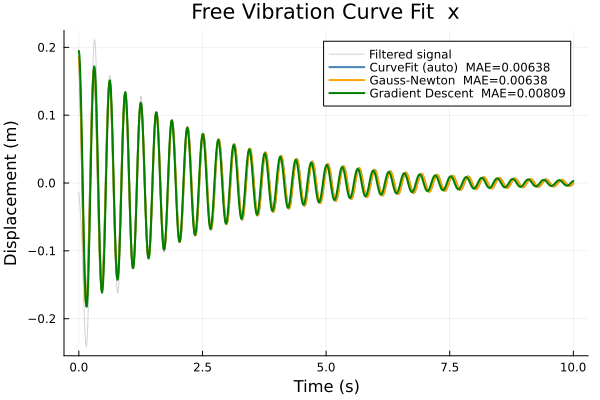
\includegraphics[width=\textwidth]{Figures/week1_approach.png}
        \caption{Week 1 Approach}
    \end{subfigure}
    \hfill
    \begin{subfigure}[b]{0.48\textwidth}
        \centering
        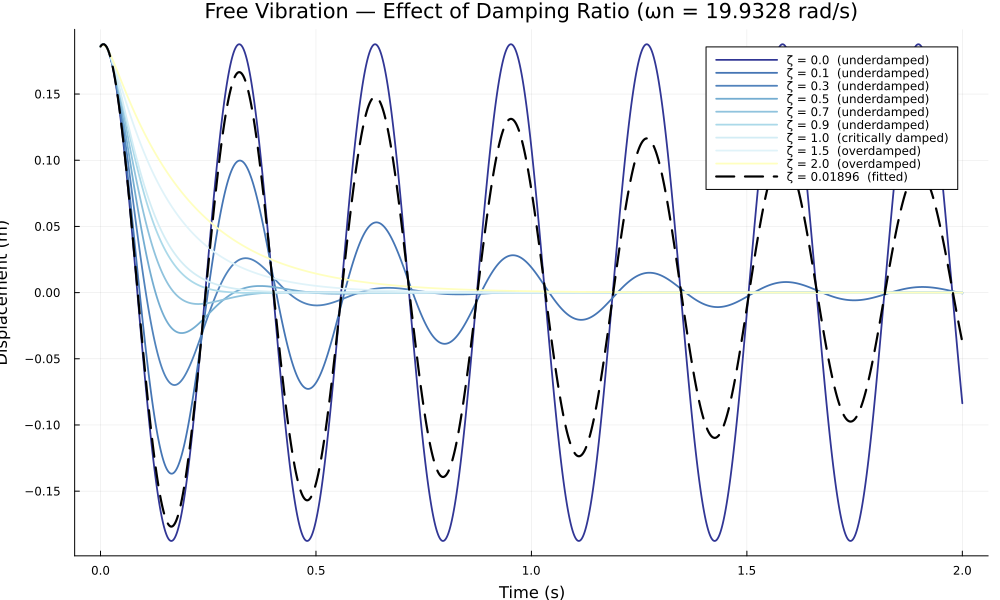
\includegraphics[width=\textwidth]{Figures/week1_change_damping.png}
        \caption{Week 1 Change Damping}
    \end{subfigure}
    \caption{X = 0.18813,$\zeta$=0.01896,$w_n$ = 19.9328, $\phi$=0.1525}
    \label{fig:week1}
\end{figure}
\subsection{2주차}
2주차에서는 1주차에서 모델링된 모델을 통해 임의의 가진에 대한 시스템의 반응, 그리고 질량 변화에 따른 시스템 거동의 변화에 대해 살펴 보았다. 아래와 같이
Diesel Rotary engine에 대한 진동에 의한 힘이 시스템에 전달 될 때 반응하는 거동을 살펴보면, 아래와 같이, 초반(transient)구간에서는 흥분현상으로 인해
큰 진폭을 보였으나, 갈수록 정상상태로 진입하여, 엔진의 진동수와 일치해가는 현상을 발견할 수 있었다. \cite{mendes2008analysis}
\begin{figure}[h!]
    \centering
    \begin{subfigure}[b]{0.21\textwidth}
        \centering
        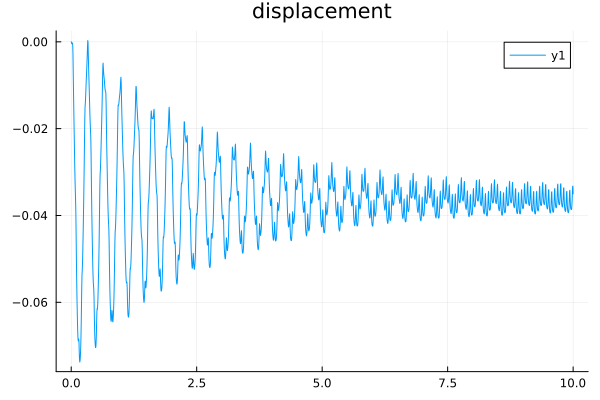
\includegraphics[width=\textwidth]{Figures/week2_only_displacement.png}
        \caption{Displacement}
    \end{subfigure}
    \hfill
    \begin{subfigure}[b]{0.21\textwidth}
        \centering
        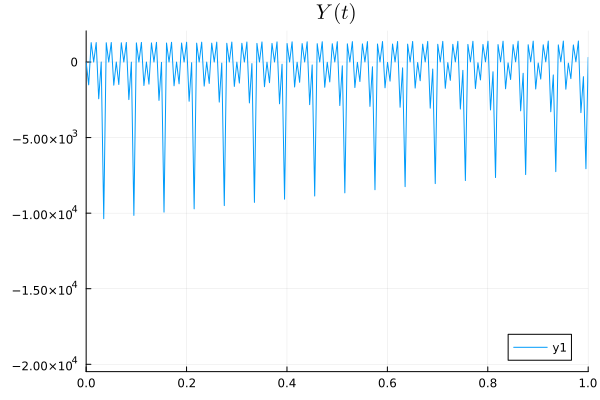
\includegraphics[width=\textwidth]{Figures/week2_only_force.png}
        \caption{Force}
    \end{subfigure}
    \hfill
    \begin{subfigure}[b]{0.21\textwidth}
        \centering
        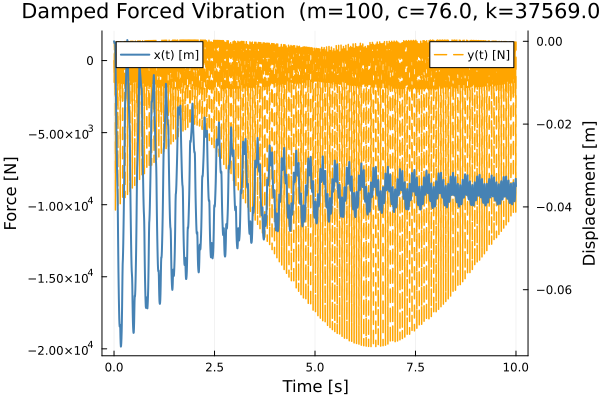
\includegraphics[width=\textwidth]{Figures/week2_total.png}
        \caption{Total}
    \end{subfigure}
    \hfill
    \begin{subfigure}[b]{0.21\textwidth}
        \centering
    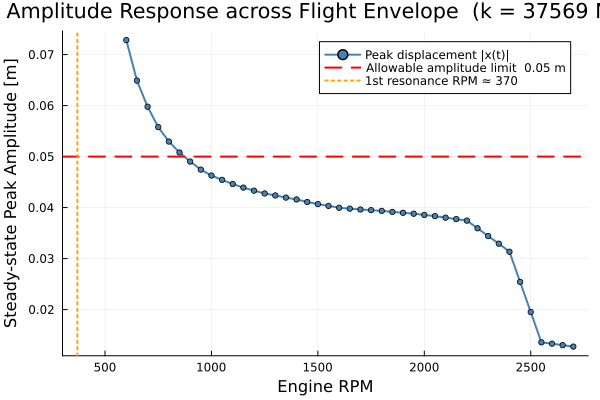
\includegraphics[width=\textwidth]{Figures/week2_rpm_relative.png}
    \caption{RPM에 따른 공진 응답}
    \end{subfigure}
    \caption{2주차 결과}
    \label{fig:week2}
\end{figure}
또한, 스프링 강성이 감소함에 따라, 1DOF의 고유주파수식, $w_n = \sqrt{k/m}$에 따라, 고유주기가 증가하는 모습을 볼 수 있었으며, 진동의 진폭또한 증가하는 것을 확인
할 수 있었다. 진폭이 증가하는 현상은 질량이 증가함에 따라 어느정도 감소하는 것을 알 수 있었다.이러한 관계(날개의 질량을 과도하게 줄이면 강성또한 낮아지며 진동으로 인한 피로가
증가함)에서, 질량과 강성 사이에 최적의 경우를 찾아야 함을 알 수 있었고, 그것을 찾기 위해 Pareto frontier와 같은 최적화 기술이 쓰임을 알 수 있었다. 또한, 이러한 관계 속에서 항공기의
연료가 탱크가 아닌 날개에 먼저 저장되는 이유도 경량화의 목적을 이루면서 날개쪽에 질량을 늘려, 피로를 줄이기 위함임을 유추 할 수 있었다. 마지막으로,
탐구 과정 도중, 위의 1DOF 모델은 아래 그림과 같이 상대적 저주파에서 공진현상을 보임을 알 수 있었다. 이로써 엔진의 과도한 idling이 연비는 아낄 수 있지만, 기체에
가하는 피로로 인해 득보다 실이 더 클 수도 있다는 것을 알게 되었다.
\subsection{3주차}
3주차부터는 위에서 서술한 2DOF 모델을 활용하여 탐구를 진행하였다. 난기류는 그 모델에 따라 \textit{von Kármán,Dryden} turbulent model 등 다양한
모델이 존재한다. 이러한 모델에서 알 수 있는 특성으로는, 난기류는 저주파 부분에서 큰 진폭을 가지며,고주파 부분은 거의 존재하지 않는다는 부분을 확인 할 수 있었다.
따라서 해당 근거에 따라서, 날개를 설계할때는 공명주파수를 너무 저주파는 아닌, 적당한 주파수 대역폭 사이에 잡아야 함을 알 수 있었다. 다만 해당 탐구에서는
보다 더 확실한 날개의 로우패스 필터의 특성을 파악하기 위해, 여러개의 사인파로 이루어진 임의의 테스트 파형을 만들어서, 그것에 대한 주파수 반응을 나타내보았다.

\begin{figure}[H] % [H] forces the figure to be placed exactly where it appears in the text
	\centering % Horizontally center the figure
	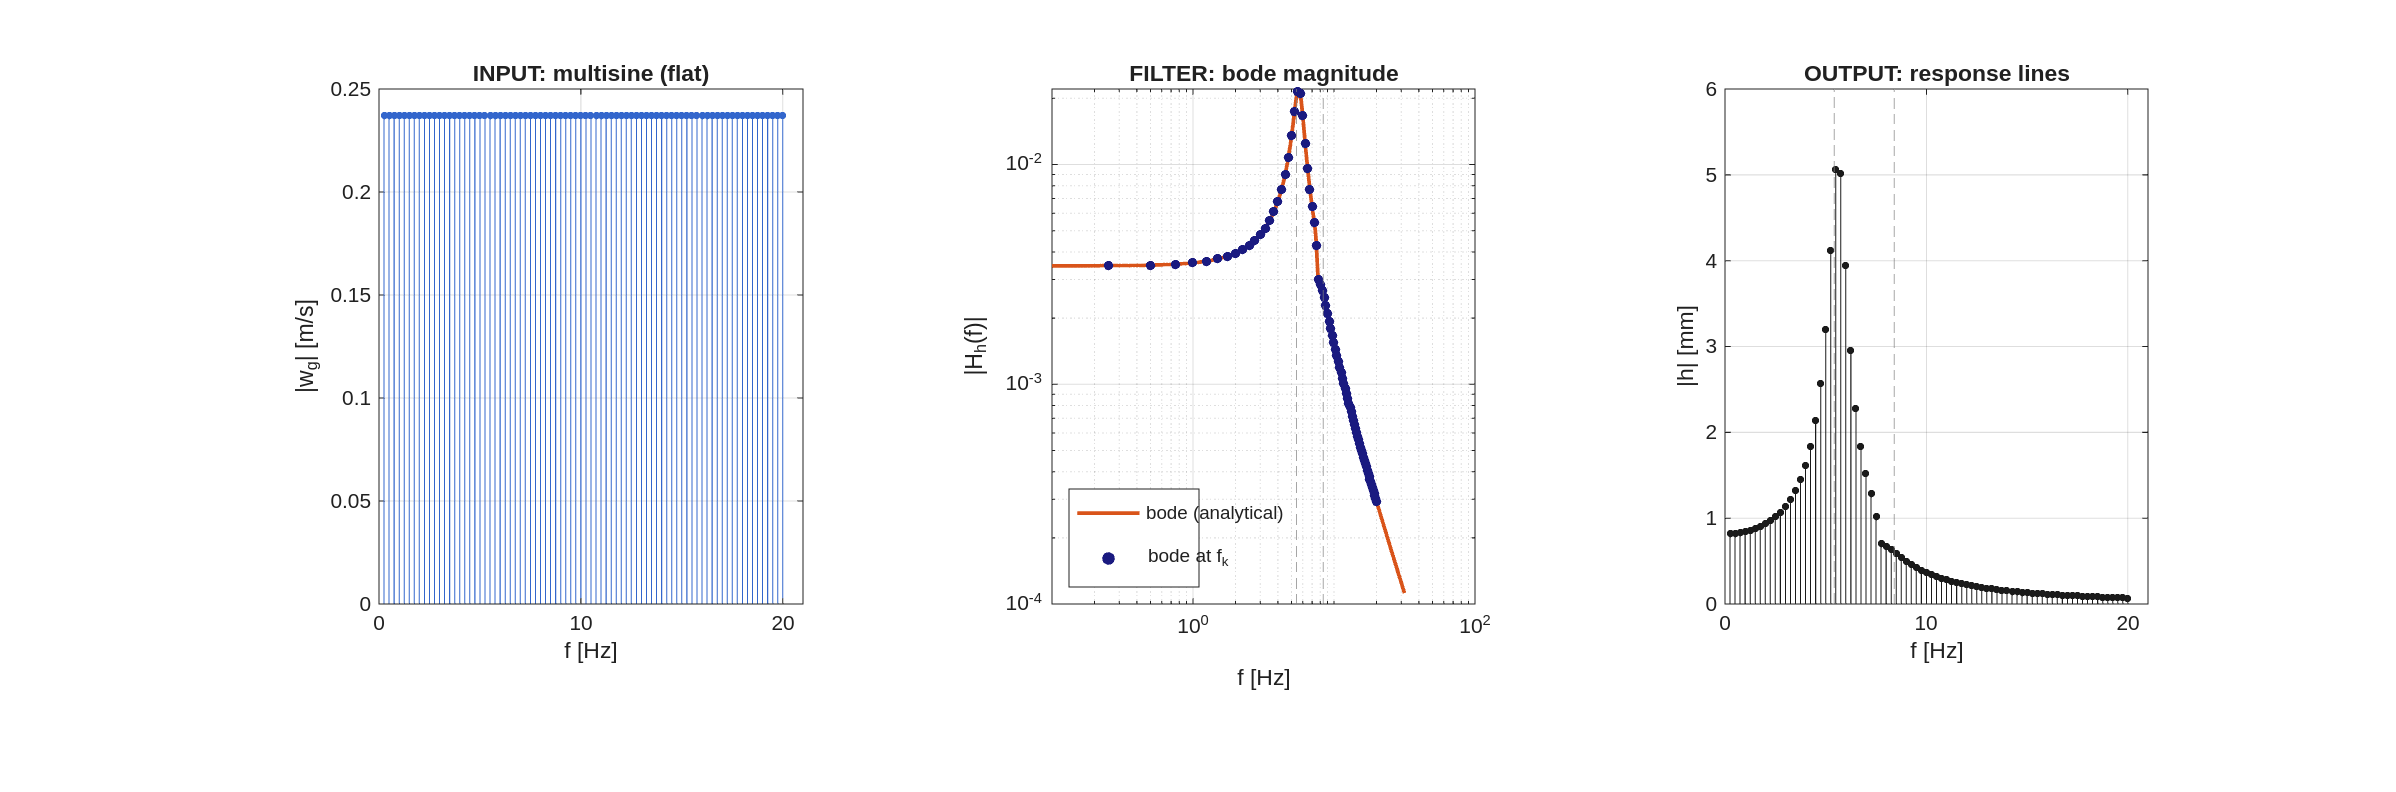
\includegraphics[width=\textwidth]{multisine_toolbox_response.png} % Include the figure
	\captionsetup{justification=centering} % Centers this specific caption
	\caption{Frequency response of sine waves with rms=1.5 }
\end{figure}

%----------------------------------------------------------------------------------------
%	BIBLIOGRAPHY
%----------------------------------------------------------------------------------------

\printbibliography % Output the bibliography

%----------------------------------------------------------------------------------------
%	Appendix
%----------------------------------------------------------------------------------------
\appendix
%======================================================================
\begin{landscape}
    \begin{multicols}{2}
\section{Structural Model from Energy}\label{sec:struct-model}
%======================================================================

\subsection{Mass Matrix --- Kinetic Energy}
Let the section have mass $m$, centre of gravity a distance $x_{\mathrm{cg}}^p$ aft
of $P$, and moment of inertia $I_{\mathrm{cg}}$ about the c.g. From \eqref{eq:kin}, the
downward velocity of the c.g. is $\dot z_{\mathrm{cg}}=\dot h + x_{\mathrm{cg}}^p\dot\theta$,
so the kinetic energy is
\begin{equation}
T = \tfrac12 m\,(\dot h + x_{\mathrm{cg}}^p\dot\theta)^2 + \tfrac12 I_{\mathrm{cg}}\dot\theta^2
  = \tfrac12 m\dot h^2 + S\,\dot h\dot\theta + \tfrac12 I_p\,\dot\theta^2 ,
\label{eq:T}
\end{equation}
where the \textbf{static unbalance} and \textbf{inertia about $P$} are defined as
\begin{equation}
S \equiv m\,x_{\mathrm{cg}}^p, \qquad I_p \equiv I_{\mathrm{cg}} + m\,({x_{\mathrm{cg}}^p})^2 .
\end{equation}
Writing $T=\tfrac12\dot{\mathbf q}^{\mathsf T}\mathbf M\dot{\mathbf q}$ with
$\mathbf q=[\,h,\ \theta\,]^{\mathsf T}$ gives
\begin{equation}
\boxed{\;\mathbf M=\begin{bmatrix} m & S\\[2pt] S & I_p \end{bmatrix}\;}
\label{eq:M}
\end{equation}
The off-diagonal $S$ represents the \emph{inertial coupling}: if the c.g. is not at $P$, plunge and
pitch exchange energy. Setting $x_{\mathrm{cg}}^p=0$ decouples them.

\subsection{Stiffness Matrix --- Spring Potential Energy}
The two springs sit at $\xi=-d/2$ (front) and $\xi=+d/2$ (rear). Their deflections are
$z_{1}=h-\tfrac{d}{2}\theta$ and $z_{2}=h+\tfrac{d}{2}\theta$, so
\begin{equation}
V=\tfrac12 k z_1^2+\tfrac12 k z_2^2
 =\tfrac12 k\!\left[\Big(h-\tfrac d2\theta\Big)^2+\Big(h+\tfrac d2\theta\Big)^2\right]
 = k\,h^2+\tfrac14 k d^2\,\theta^2 .
\label{eq:V}
\end{equation}
The cross terms $\mp d\,h\theta$ cancel because $P$ is the midpoint. With
$V=\tfrac12\mathbf q^{\mathsf T}\mathbf K_s\mathbf q$,
\begin{equation}
\boxed{\;\mathbf K_s=\begin{bmatrix} 2k & 0\\[2pt] 0 & \tfrac12 k d^2 \end{bmatrix}\;}
\label{eq:Ks}
\end{equation}
i.e., plunge stiffness $2k$ and pitch stiffness $\tfrac12 kd^2$.

\subsection{Damping Matrix --- Rayleigh Dissipation}
The dampers act in parallel with the springs, so the Rayleigh dissipation function is
identical in form to \eqref{eq:V} with $k\!\to\!c$ and $z\!\to\!\dot z$:
$\mathcal D=\tfrac12 c\dot z_1^2+\tfrac12 c\dot z_2^2$, giving\footnote{For a viscous damper $F_{v}=c\dot{z}$, the Rayleigh dissipation function is $\mathcal{D}=\frac{1}{2}c\dot{z}^{2}$, which represents half the rate of energy dissipation (power) of the system.}
\begin{equation}
\boxed{\;\mathbf C=\begin{bmatrix} 2c & 0\\[2pt] 0 & \tfrac12 c d^2 \end{bmatrix}\;}
\label{eq:C}
\end{equation}
This term is essential: without it, the resonance peaks would be infinite; a few percent of critical
damping makes them finite and realistic.

\subsection{Structural Equations of Motion}
Lagrange's equations,
$\frac{d}{dt}\!\big(\partial T/\partial\dot q_i\big)-\partial T/\partial q_i
+\partial V/\partial q_i+\partial\mathcal D/\partial\dot q_i=Q_i$,
yield
\begin{equation}
\mathbf M\ddot{\mathbf q}+\mathbf C\dot{\mathbf q}+\mathbf K_s\mathbf q=\mathbf Q_{\text{aero}},
\label{eq:struct-eom}
\end{equation}
where $\mathbf Q_{\text{aero}}$ denotes the generalised aerodynamic forces derived next.

\subsection{Aerodynamic Forces}
The lift acts at the aerodynamic centre, a distance $e_a$ \emph{forward} of $P$
(i.e., $\xi_{\mathrm{ac}}=-e_a$). A vertical gust of velocity $w_g$ adds an incremental
angle of attack $w_g/U$ to the geometric pitch $\theta$, where $U$ is the flight speed.
Furthermore, when the wing plunges downward at velocity $\dot{h}$, it experiences an upward relative wind, 
creating an induced angle of attack of $\frac{\dot{h}}{U}$. Under the quasi-steady approximation, lift is proportional to the effective angle
of attack through $C_{l\alpha}$:
\begin{equation}
L = \bar{q} S\, C_{l\alpha}\Big(\theta +\frac{\dot{h}}{U} + \frac{w_g}{U}\Big),
\qquad \bar{q} S = \tfrac{1}{2}\rho U^2 c\, b
\label{eq:lift}
\end{equation}
For a NACA~2412 airfoil, $C_{l\alpha}\approx 2\pi$, and $\bar{q} S$ is the dynamic
pressure multiplied by the planform area.\footnote{The unsteady Theodorsen/Sears
corrections are omitted. this slightly overestimates the
peaks but is appropriate for the present reduced-order model.}
The virtual work of the upward lift
under a virtual displacement of $P$ gives the generalised forces:
\begin{equation}
Q_h=-L,\qquad Q_\theta=+L\,e_a ,
\label{eq:Q}
\end{equation}
The constant aerodynamic-centre moment $M_{\mathrm{ac}}$ only shifts the trim and is dropped
from the dynamics.Splitting \eqref{eq:lift} into a part driven by the motion ($\theta$, $\dot{h}$, $\dot{\theta}$) and a
part driven by the gust $w_g$,
\begin{equation}
\begin{bmatrix}Q_h\\ Q_\theta\end{bmatrix}
=\underbrace{\bar{q} S\,C_{l\alpha}\begin{bmatrix}0&-1\\0&\ e_a\end{bmatrix}
\begin{bmatrix}h\\ \theta\end{bmatrix}
+\frac{\bar{q} S\,C_{l\alpha}}{U} \begin{bmatrix} -1 & 0 \\ e_a & 0 \end{bmatrix} \begin{bmatrix} \dot{h} \\ \dot{\theta} \end{bmatrix}}_{\text{motion-dependent}}
+\underbrace{\frac{\bar{q} S\,C_{l\alpha}}{U}\begin{bmatrix}-1\\ e_a\end{bmatrix}w_g}_{\text{gust forcing}} .
\end{equation}
Moving the motion-dependent part to the left of \eqref{eq:struct-eom} defines the
\textbf{aerodynamic stiffness} $\mathbf K_a$, \textbf{aerodynamic damping} $\mathbf C_a$, and \textbf{gust force vector} $\mathbf F_g$:
\begin{equation}
\boxed{\ \mathbf K_a = \bar{q} S\, C_{l\alpha}\!
\begin{bmatrix} 0 & 1 \\ 0 & -e_a \end{bmatrix},\qquad
\mathbf C_a = \frac{\bar{q} S\, C_{l\alpha}}{U}\!
\begin{bmatrix} 1 & 0 \\ -e_a & 0 \end{bmatrix},\qquad
\mathbf F_g = \frac{\bar{q} S\, C_{l\alpha}}{U}\!
\begin{bmatrix} -1 \\ e_a \end{bmatrix}.\ }
\end{equation}
Note that $\mathbf K_a$ is \emph{not} symmetric: aerodynamic loads are
non-conservative follower forces. This asymmetry is harmless at low speed but is
the very mechanism that produces flutter at high speed.

\subsection{Assembled System}
Collecting everything, the governing equation \eqref{eq:struct-eom} becomes
\begin{equation}
\boxed{\ \mathbf M\,\ddot{\mathbf q}
+ \big(\mathbf C + \mathbf C_a\big)\,\dot{\mathbf q}
+ \big(\mathbf K_s + \mathbf K_a\big)\,\mathbf q
= \mathbf F_g\, w_g(t).\ }
\label{eq:eom}
\end{equation}
% Compromise them all, then the matrix are shown as below.\cref{tab:matrices}
% \begin{table}[h]
% \centering
% \caption{System matrices ($\bar{q}S = \tfrac{1}{2}\rho U^2 c\,b$)}
% \label{tab:matrices}
% \renewcommand{\arraystretch}{1.4}
% \begin{tabular}{ll}
% \toprule
% Matrix & Definition \\
% \midrule
% $\mathbf{M}$
%   & $\begin{bmatrix} m & S \\ S & I_p \end{bmatrix}$ \\[6pt]
% $\mathbf{C}$
%   & $\begin{bmatrix} 2c_d & 0 \\ 0 & \tfrac{1}{2}c_d d^2 \end{bmatrix}$,\quad
%     $\mathbf{C}_a = \dfrac{\bar{q}S\,C_{l\alpha}}{U}
%     \begin{bmatrix} 1 & 0 \\ -e_a & 0 \end{bmatrix}$ \\[6pt]
% $\mathbf{K}_s$
%   & $\begin{bmatrix} 2k & 0 \\ 0 & \tfrac{1}{2}k d^2 \end{bmatrix}$,\quad
%     $\mathbf{K}_a = \bar{q}S\,C_{l\alpha}
%     \begin{bmatrix} 0 & 1 \\ 0 & -e_a \end{bmatrix}$ \\[6pt]
% $\mathbf{F}_g$
%   & $\dfrac{\bar{q}S\,C_{l\alpha}}{U}\begin{bmatrix} -1 \\ e_a \end{bmatrix}$ \\
% \bottomrule
% \end{tabular}
% \end{table}
%----------------------------------------------------------------------------------------
    \end{multicols}
\end{landscape}
\end{document}